\documentclass[11pt]{article}
\usepackage[margin=1in]{geometry}
\usepackage[T1]{fontenc}
\usepackage{lmodern}
\usepackage{amsmath}
\usepackage{graphicx}
\usepackage{float}
\usepackage{booktabs}
\usepackage{hyperref}
\usepackage{xcolor}
\usepackage{listings}

\lstdefinelanguage{MIPS}{
  morekeywords={
    add,addu,addi,addiu,and,andi,
    beq,bne,div,divu,j,jal,jr,la,lb,lbu,lh,lhu,
    li,lui,lw,mfhi,mflo,move,mult,multu,nop,nor,or,ori,
    sb,sh,sw,sll,sllv,slt,slti,sltiu,sltu,sra,srl,sub,subu,syscall,
    xor
  },
  sensitive=true,
  morecomment=[l]{\#},
  morestring=[b]"
}

\lstset{
  basicstyle=\ttfamily\small,
  keywordstyle=\color{blue!60!black},
  commentstyle=\color{gray!70},
  stringstyle=\color{green!40!black},
  numbers=left,
  numberstyle=\tiny\color{gray!70},
  stepnumber=1,
  numbersep=8pt,
  tabsize=4,
  showstringspaces=false,
  breaklines=true,
  captionpos=b
}

\title{EE161 Lab 1 Report\\Hands-on with the MIPS ISA using MARS}
\author{Kaushik Vada (vvada002)}
\date{\today}

\begin{document}
\maketitle

\section{Part 1 -- Registers and Arithmetic}
\subsection*{Objectives}
Swap two register values without a temporary register, then compute arithmetic operations on the swapped operands while observing the resulting register file state.

\subsection*{Implementation Details}
I used an XOR-swapping sequence to exchange the values in \texttt{\$t0} and \texttt{\$t1}, guaranteeing no additional registers were required. After the swap, the program performs addition, subtraction, and multiplication, storing the results in \texttt{\$t2}, \texttt{\$t3}, and \texttt{\$t4}. The multiplication result is retrieved from \texttt{LO} via \texttt{mflo}.

\begin{lstlisting}[language=MIPS, caption={Part~1 solution (\texttt{part1\_Solution.asm})}, label=lst:part1]
# Lab 1: Registers and Arithmetic Operations

.data
    num1: .word 5
    num2: .word 10

.text
    lw $t0, num1
    lw $t1, num2

    xor  $t0, $t0, $t1
    xor  $t1, $t0, $t1
    xor  $t0, $t0, $t1

    addu $t2, $t0, $t1
    subu $t3, $t0, $t1

    mult $t0, $t1
    mflo $t4

    li $v0, 10
    syscall
\end{lstlisting}

\subsection*{Results}
Swapping the loaded constants of 5 and 10 results in \texttt{\$t0 = 10} and \texttt{\$t1 = 5}. The computed outputs are \texttt{\$t2 = 15}, \texttt{\$t3 = 5}, and \texttt{\$t4 = 50}, matching the expected arithmetic outcomes. The captured register window in Figure~\ref{fig:part1} confirms these values inside MARS.

\begin{figure}[H]
  \centering
  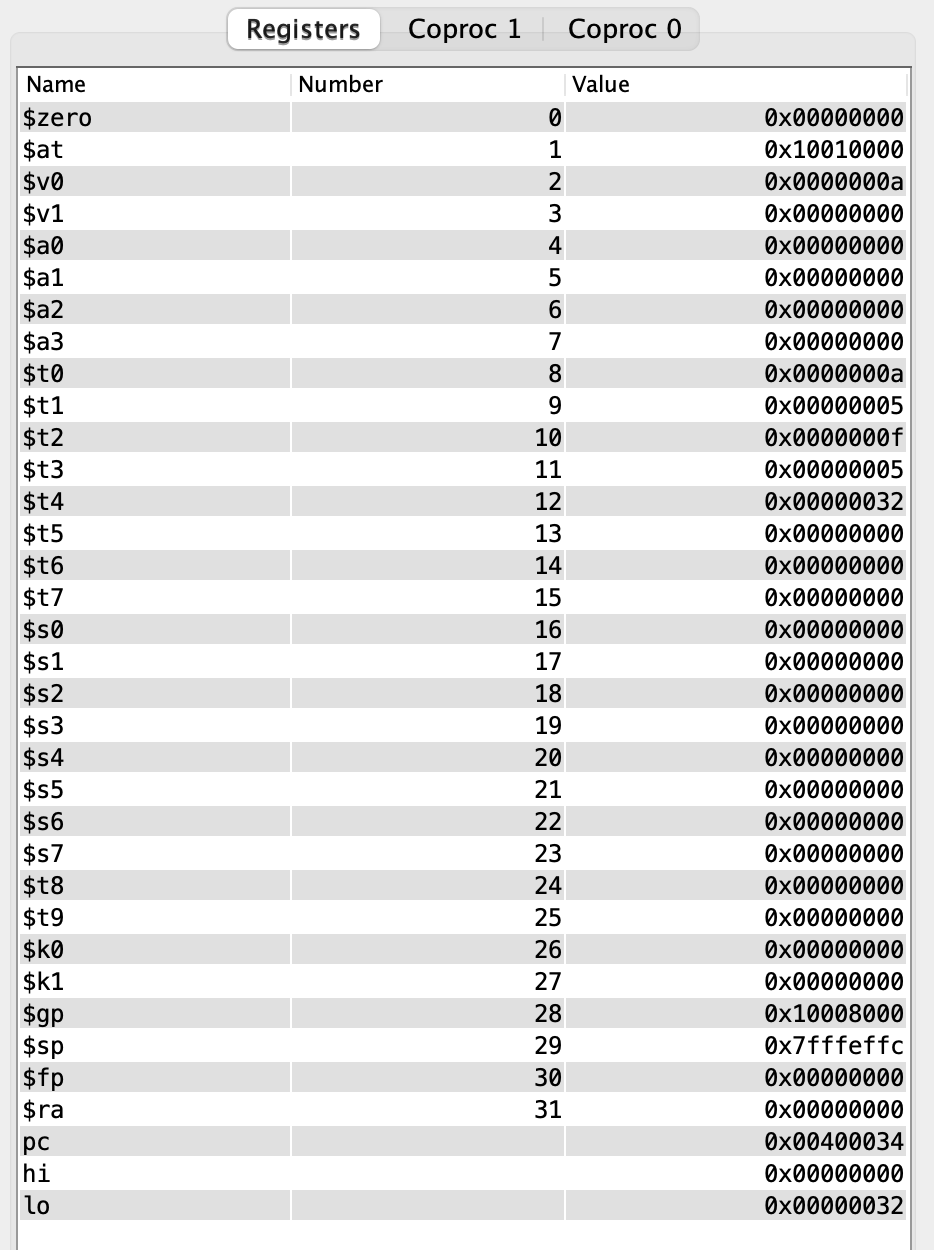
\includegraphics[width=0.55\linewidth]{part1-register.png}
  \caption{Register state after executing Part~1 program.}
  \label{fig:part1}
\end{figure}

\newpage
\section{Part 2 -- Debugging a Loop and Working with Arrays}
\subsection*{Objectives}
Repair the provided loop so it correctly iterates across an array, accumulate the original sum, double each element in place, and track the maximum doubled value.

\subsection*{Bug Analysis and Fix}
The starter loop failed to advance the base address by a full word and attempted to load using a malformed pseudo-instruction, effectively rereading the same element and leaving the pointer misaligned. Replacing the invalid operation with a proper \texttt{lw} from \texttt{0(\$t0)} and incrementing the pointer using \texttt{addi \$t0, \$t0, 4} restored correct traversal. This change ensures each iteration reads the intended element, updates it, and proceeds to the next address boundary.

\subsection*{Implementation Details}
The corrected program sums the original array into \texttt{\$t2}, doubles each element using a left shift, and tracks the maximum doubled result with a compare-and-select pattern. After the loop, it writes the computed sum and maximum to memory so they can be inspected from the data segment.

\begin{lstlisting}[language=MIPS, caption={Part~2 solution (\texttt{part2\_Solution.asm})}, label=lst:part2]
# Lab 2 Starter Code: Debugging a Loop

.data
    arr:     .word 1, 4, 7, 2, 5
    n:       .word 5
    result:  .word 0
    maxval:  .word 0

.text
.globl main
main:
    la   $t0, arr
    lw   $t1, n
    li   $t2, 0
    li   $t5, 0x80000000

loop:
    beq  $t1, $zero, done
    lw   $t3, 0($t0)

    addu $t2, $t2, $t3

    sll  $t4, $t3, 1
    sw   $t4, 0($t0)

    slt  $t6, $t5, $t4
    beq  $t6, $zero, skip_max
    move $t5, $t4
skip_max:
    addi $t0, $t0, 4
    addi $t1, $t1, -1
    j    loop

done:
    sw   $t2, result
    sw   $t5, maxval

    li   $v0, 10
    syscall
\end{lstlisting}

\subsection*{Results}
The original sum of the array is 19, while the doubled array becomes \{2, 8, 14, 4, 10\}. The maximum doubled value is 14. These values agree with the expectations and the data segment snapshot in Figure~\ref{fig:part2}. A quick summary is provided in Table~\ref{tab:part2-results}.

\begin{table}[H]
  \centering
  \caption{Computed metrics for Part~2.}
  \label{tab:part2-results}
  \begin{tabular}{lc}
    \toprule
    Quantity & Value \\
    \midrule
    Sum of original elements & 19 \\
    Doubled array & $\{2, 8, 14, 4, 10\}$ \\
    Maximum doubled value & 14 \\
    \bottomrule
  \end{tabular}
\end{table}

\begin{figure}[H]
  \centering
  \includegraphics[width=0.50\linewidth]{{part 2-register}.png}
  \caption{MARS output showing doubled array, sum, and maximum value.}
  \label{fig:part2}
\end{figure}

\newpage
\section{Part 3 -- Stack and Function Call Simulation}
\subsection*{Objectives}
Finalize the provided function template so it obeys the MIPS calling convention, uses the stack to protect caller state, and demonstrates multiple calls that store returned results.

\subsection*{Implementation Details}
The \texttt{sum} procedure now allocates a four-byte stack frame, saves the return address (\texttt{\$ra}), and restores it prior to returning. The main routine issues two calls with different argument pairs, storing each result in memory locations \texttt{result} and \texttt{result2}. This sequence validates that \texttt{\$v0} is successfully returned and that the stack is balanced across calls.

\begin{lstlisting}[language=MIPS, caption={Part~3 solution (\texttt{part3\_Solution.asm})}, label=lst:part3]
# Lab 3 Starter Code: Stack and Function Call Simulation

.data
    result:  .word 0
    result2: .word 0

.text
main:
    li $a0, 5
    li $a1, 10
    jal sum
    move $t0, $v0
    sw $v0, result

    li $a0, 12
    li $a1, 7
    jal sum
    move $t1, $v0
    sw $v0, result2

    li $v0, 10
    syscall

sum:
    addiu $sp, $sp, -4
    sw $ra, 0($sp)

    addu $v0, $a0, $a1

    lw $ra, 0($sp)
    addiu $sp, $sp, 4
    jr $ra
\end{lstlisting}

\newpage
\subsection*{Results}
The function returns 15 for the first call and 19 for the second, corresponding to the provided argument pairs. Figure~\ref{fig:part3} captures the register and memory view that verifies both stored results. The explicit push/pop of \texttt{\$ra} ensures the return address survives nested calls, illustrating the core idea behind stack frames: reserving space for saved registers and local data while maintaining balanced stack pointer adjustments.

\begin{figure}[H]
  \centering
  \includegraphics[width=0.55\linewidth]{{part 3-register}.png}
  \caption{Register and memory snapshot after executing both function calls.}
  \label{fig:part3}
\end{figure}

\section{Discussion and Lessons Learned}
This lab reinforced several foundational ISA competencies: using bitwise operations to eliminate temporary storage, reasoning about pointer arithmetic and memory alignment, and adhering to calling conventions via explicit stack management. Validating each stage in MARS highlighted how quickly small instruction-level mistakes (such as incorrect pointer increments) propagate through a program, underscoring the value of careful register and memory inspection. The resulting assembly artifacts and screenshots provide a complete record of the working solutions.

\end{document}
